\documentclass[handout]{beamer}
\usetheme[titleprogressbar]{m}

%\usepackage{pgfpages}
%%\setbeameroption{show notes}
%\setbeameroption{show notes on second screen=right}

\setbeamertemplate{caption}[numbered]

\usepackage{tikz}
\usetikzlibrary{calc, matrix, arrows, arrows.meta, automata, shapes, positioning, shadows, trees}

\definecolor{myyellow}{RGB}{240,217,1}
\definecolor{mygreen}{RGB}{143,188,103}
\definecolor{myred}{RGB}{234,38,40}
\definecolor{myblue}{RGB}{53,101,167}

\usepackage{graphicx}
\usepackage{multimedia}
%\usepackage[latin1]{inputenc}
\setbeamercovered{transparent}
\usepackage{pgfplots}
\usepackage{pgfplotstable}
\usepackage{color}
\usepackage{subfigure}

\tikzset{basic/.style={draw}}
\tikzset{input/.style={basic, circle}}
\tikzset{bias/.style={basic, rectangle}}
\tikzset{neuron/.style={basic, circle}}
\tikzset{>=stealth, font=\scriptsize}
\tikzset{sectors/.style n args={2}{%
     circle, draw, minimum width=3.444em,
     append after command={%
         \pgfextra{ %
            \draw (\tikzlastnode.north) -- (\tikzlastnode.south);
            \path (\tikzlastnode.center) -- node[] {#1} (\tikzlastnode.west);
            \path (\tikzlastnode.center) -- node[] {#2} (\tikzlastnode.east);
         }
      }
   }
}

% Beamer stuff
\newcommand\ppbb{path picture bounding box}
\setbeamerfont{bibliography item}{size=\tiny}
\setbeamerfont{bibliography entry author}{size=\tiny}
\setbeamerfont{bibliography entry title}{size=\tiny}
\setbeamerfont{bibliography entry location}{size=\tiny}
\setbeamerfont{bibliography entry note}{size=\tiny}


% argmin
\newcommand{\argmin}[1]{\underset{#1}{\operatorname{arg}\,\operatorname{min}}\;}
% argmax
\newcommand{\argmax}[1]{\underset{#1}{\operatorname{arg}\,\operatorname{max}}\;}

\title[\insertdate]{From Linear Algebra\\to Machine Learning}

\author{Omar Guti\'errez}
\institute{@trinogz}
\date{\today}

\begin{document}

\maketitle

\begin{frame}
    \frametitle{Overview}
    \tableofcontents
\end{frame}


\section{Motivation}
\begin{frame}{Motivation}
    \begin{itemize}
        \item \textbf{Linear algebra} is important to understand machine learning.
        \item As well as \textbf{calculus}, \textbf{probability theory}, and \textbf{statistics}.
        \item It is rewarding to take the \textbf{hard path} to learn machine learning (IMHO).
    \end{itemize}
\end{frame}


\begin{frame}{Learning from errors}
    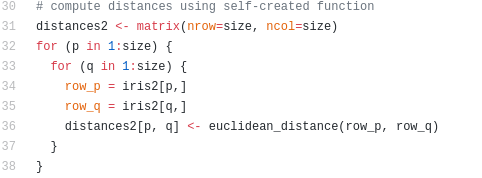
\includegraphics[scale=0.555]{figures/naive_distance_matrix_r.png}
\end{frame}


\begin{frame}{Learning from errors}
    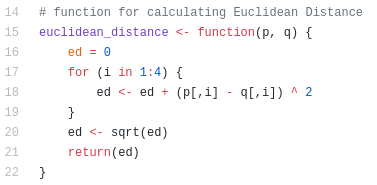
\includegraphics[scale=0.555]{figures/naive_euclidean_r.png}
\end{frame}


%    columns
%    \begin{columns}
%        %%%%%%%%%%%%%%%%%%%%%%%%%%%%%%%%%%%%%%%%%%%%%%%%%%%%%%%%%%%%%%%%%%%%%%
%        \begin{column}{0.5\textwidth}
%        \end{column}
%
%        %%%%%%%%%%%%%%%%%%%%%%%%%%%%%%%%%%%%%%%%%%%%%%%%%%%%%%%%%%%%%%%%%%%%%%
%        \begin{column}{0.5\textwidth}
%        \end{column}
%
%    \end{columns}


\section{Vectors}
%\subsection{Length of a vector}
\begin{frame}{A vector is a collection of numbers}
    \Huge
    \begin{align*} 
        \textcolor{blue}{\vec{a} = \boldsymbol{a}} &= \begin{bmatrix}
           a_{1}  \\
           a_{2}  \\
           \vdots \\
           a_{n}  
         \end{bmatrix}
    \end{align*}
\end{frame}


\begin{frame}{Length of a vector}
    \huge
    \begin{align*}
        \textcolor{blue}{|\boldsymbol{a}|}   &= \sqrt{\sum^{n}_{i=1} a_i^2}
        %\textcolor{blue}{
        %||\boldsymbol{x}||_p = \Bigg(\sum^{n}_{i=1} |x_i|^p\Bigg)^\frac{1}{p}
        %}
    \end{align*}
\end{frame}
\note{
    \begin{itemize}
        \item remark that sometimes vectors have a symbol above, or are written in bold letters
    \end{itemize}
}

%\subsection{Distance}
\begin{frame}{Distance beetwen vectors}
    \Large
    \begin{align*}
        d(\boldsymbol{a}, \boldsymbol{b}) &= ||\boldsymbol{a} - \boldsymbol{b}||\\
                                          &= \sqrt{\sum_{i=0}^n (a_{i} - b_{i})^2}
    \end{align*}
\end{frame}


%\subsection{Dot product}
\begin{frame}{Dot product}
    \Large
    \begin{align*}
        \textcolor{red}{a \cdot b} &= \textcolor{brown}{\sum_{i=0}^{n} a_i b_i} \\
                                   &= \textcolor{blue}{a_0b_0 + a_1b_1 + \ldots + a_nb_n}
    \end{align*}
    So,
    \begin{align*}
        \textcolor{red}{a \cdot a} &= a_0a_0 + a_1a_1 + \ldots + a_na_n \\
                                   &= a_0^2  + a_1^2  + \ldots + a_n^2 \\
                                   &= |\boldsymbol{a}|^2
    \end{align*}
\end{frame}

\section{Examples}
%\subsection{Perceptron}
{
\usebackgroundtemplate{
\includegraphics[width=\paperwidth, height=\paperheight]{figures/winter-is-coming.jpg}}%
\begin{frame}{}
\end{frame}
}

\begin{frame}{The AI winter is coming}
    \begin{itemize}
        \item Is really coming? No.
        \item However, we already had an AI winter.
        \item The research on neural nets was stopped for many years, after
                Minsky and Papert proved that a single layer perceptron was not able to
                deal with the exclusive-or problem.
    \end{itemize}
\end{frame}

\begin{frame}[fragile]
    \frametitle{Linear Regression}
    \begin{figure}[htb]
        \centering
        \pgfmathsetseed{1138} % set the random seed
\pgfplotstableset{ % Define the equations for x and y
    create on use/x/.style={create col/expr={42+2*\pgfplotstablerow}},
    create on use/y/.style={create col/expr={(0.6*\thisrow{x}+130)+5*rand}}
}
% create a new table with 30 rows and columns x and y:
\pgfplotstablenew[columns={x,y}]{30}\loadedtable

% Calculate the regression line
\pgfplotstablecreatecol[linear regression]{regression}{\loadedtable}

\pgfplotsset{
    colored residuals/.style 2 args={
        only marks,
        scatter,
        point meta=explicit,
        colormap={redblue}{color=(#1) color=(#2)},
        error bars/y dir=minus,
        error bars/y explicit,
        error bars/draw error bar/.code 2 args={
            \pgfkeys{/pgf/fpu=true}
            \pgfmathtruncatemacro\positiveresidual{\pgfplotspointmeta<0}
            \pgfkeys{/pgf/fpu=false}
            \ifnum\positiveresidual=0
                \draw [#2] ##1 -- ##2;
            \else
                \draw [#1] ##1 -- ##2;
            \fi
        },
        /pgfplots/table/.cd,
            meta expr=(\thisrow{y}-\thisrow{regression})/abs(\thisrow{y}-\thisrow{regression}),
            y error expr=\thisrow{y}-\thisrow{regression}
    },
    colored residuals/.default={brown}{brown}
}

\begin{tikzpicture}
\begin{axis}[
xlabel=x, % label x axis
ylabel=y, % label y axis
axis lines=left, %set the position of the axes
xmin=40, xmax=105, % set the min and max values of the x-axis
ymin=150, ymax=200, % set the min and max values of the y-axis
]

\makeatletter
\addplot [colored residuals] table {\loadedtable};
\addplot [
    no markers,
    thick, black
] table [y=regression] {\loadedtable} ;
\end{axis}

\end{tikzpicture}

        \label{fig:regression}
	\end{figure}
\end{frame}

\begin{frame}[fragile]
    \frametitle{Linear Regression}
    \Large
    \begin{itemize}
        \item We want to calculate the intercept $a$ and the slope $b$.
    \end{itemize}
    \begin{align*}
        \argmin{a, b} \sum_i (y_i - (ax_i + b))^2 =
        \argmin{\boldsymbol{w}} || \boldsymbol{Xw} - \boldsymbol{y} ||^{2}
    \end{align*}
    \begin{itemize}
        \item The solution to this optimization problem is:
    \end{itemize}
    \begin{align*}
        \boldsymbol{w^{*}} = (\boldsymbol{X}^T\boldsymbol{X})^{-1}\boldsymbol{X}^{T}\boldsymbol{y}\,.
    \end{align*}
\end{frame}

%\begin{frame}[fragile]\frametitle{Toy dataset}
%    \begin{figure}[htb]
%        \centering
%        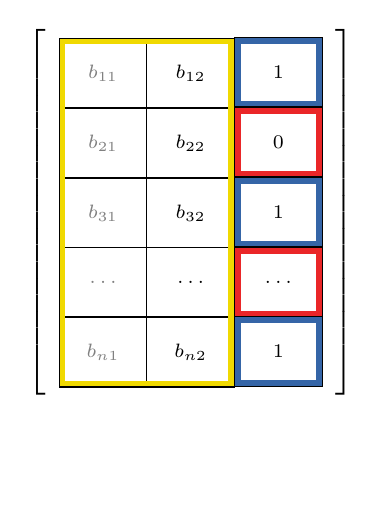
\begin{tikzpicture}[
mymatrix/.style={
  matrix of math nodes,
  outer sep=0pt,
  nodes={
    draw,
    text width=2.5em,
    align=center,
    minimum height=2.5em,
    text=gray
  },
  nodes in empty cells,
  column sep=-\pgflinewidth,
  row sep=-\pgflinewidth,
  left delimiter=[,
  right delimiter=],
  },
  mycircle/.style 2 args={
    draw=#1,
    circle,
    fill=#2,
    line width=2pt,
    inner sep=5pt
  },
  arr/.style={
  line width=4pt,
  -{Triangle[angle=60:1.5pt 3]},
  #1,
  shorten >= 3pt,
  shorten <= 3pt
  }
]
%the matrices
\matrix[mymatrix,anchor=south west] (B)
{
b_{11} & |[text=black]|b_{12} & |[text=black]| 1 \\
b_{21} & |[text=black]|b_{22} & |[text=black]| 0 \\
b_{31} & |[text=black]|b_{32} & |[text=black]| 1 \\
\ldots & |[text=black]|\ldots & |[text=black]| \ldots \\
b_{n1} & |[text=black]|b_{n2} & |[text=black]| 1 \\
};

%the frames in both matrices
\draw[myyellow,line width=2pt]
  ([shift={(1.2pt,-1.2pt)}]B-1-1.north west) 
  rectangle 
  ([shift={(-1.2pt,1.2pt)}]B-5-2.south east);

\draw[myblue,line width=2pt]
  ([shift={(1.2pt,-1.2pt)}]B-1-3.north west) 
  rectangle 
  ([shift={(-1.2pt,1.2pt)}]B-1-3.south east);

\draw[myred,line width=2pt]
  ([shift={(1.2pt,-1.2pt)}]B-2-3.north west) 
  rectangle 
  ([shift={(-1.2pt,1.2pt)}]B-2-3.south east);

\draw[myblue,line width=2pt]
  ([shift={(1.2pt,-1.2pt)}]B-3-3.north west) 
  rectangle 
  ([shift={(-1.2pt,1.2pt)}]B-3-3.south east);

\draw[myred,line width=2pt]
  ([shift={(1.2pt,-1.2pt)}]B-4-3.north west) 
  rectangle 
  ([shift={(-1.2pt,1.2pt)}]B-4-3.south east);

\draw[myblue,line width=2pt]
  ([shift={(1.2pt,-1.2pt)}]B-5-3.north west) 
  rectangle 
  ([shift={(-1.2pt,1.2pt)}]B-5-3.south east);

%the legend
\matrix[
  matrix of math nodes,
  nodes in empty cells,
  column sep=10pt,
  anchor=north,
  nodes={
    minimum height=2.2em,
    minimum width=2em,
    anchor=north west
  },
  below=5pt of current bounding box.south
  ] 
  (legend) {\\};

\end{tikzpicture}

%        \label{fig:toy}
%	\end{figure}
%\end{frame}
%
%\begin{frame}[fragile]\frametitle{What is happening?}
%    \begin{figure}[htb]
%		\centering
%		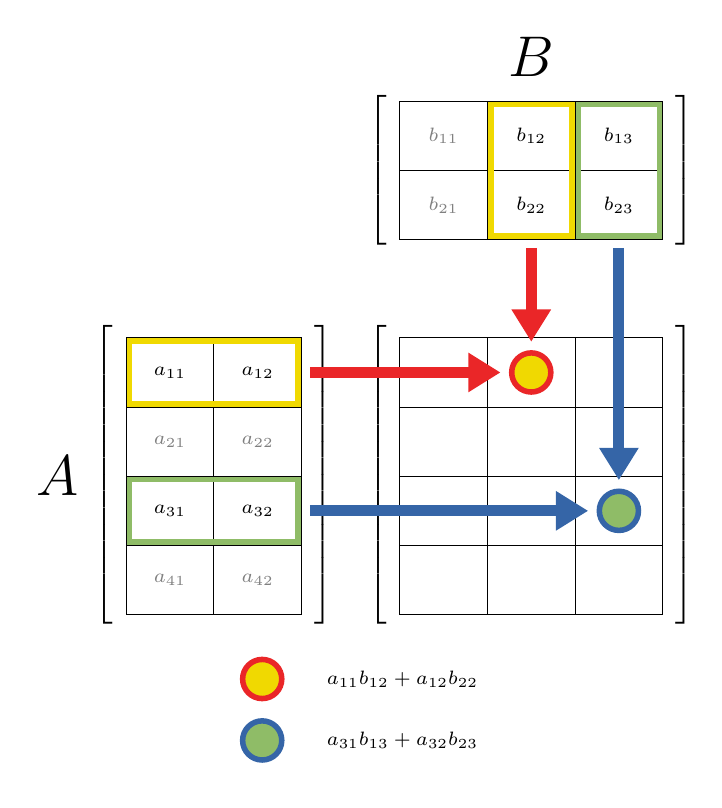
\begin{tikzpicture}[
mymatrix/.style={
  matrix of math nodes,
  outer sep=0pt,
  nodes={
    draw,
    text width=2.5em,
    align=center,
    minimum height=2.5em,
    text=gray
  },
  nodes in empty cells,
  column sep=-\pgflinewidth,
  row sep=-\pgflinewidth,
  left delimiter=[,
  right delimiter=],
  },
  mycircle/.style 2 args={
    draw=#1,
    circle,
    fill=#2,
    line width=2pt,
    inner sep=5pt
  },
  arr/.style={
  line width=4pt,
  -{Triangle[angle=60:1.5pt 3]},
  #1,
  shorten >= 3pt,
  shorten <= 3pt
  }
]
%the matrices
\matrix[mymatrix] (A)
{
|[text=black]|a_{11} & |[text=black]|a_{12} \\
a_{21} & a_{22} \\
|[text=black]|a_{31} & |[text=black]|a_{32} \\
a_{41} & a_{42} \\
};
\matrix[mymatrix,right=of A.north east,anchor=north west] (prod)
{
& & \\
& & \\
& & \\
& & \\
};
\matrix[mymatrix,above=of prod.north west,anchor=south west] (B)
{
b_{11} & |[text=black]|b_{12} & |[text=black]|b_{13} \\
b_{21} & |[text=black]|b_{22} & |[text=black]|b_{23} \\
};

%the labels for the matrices
\node[font=\huge,left=10pt of A] {$A$};
\node[font=\huge,above=2pt of B] {$B$};

%the frames in both matrices
\draw[myyellow,line width=2pt]
  ([shift={(1.2pt,-1.2pt)}]A-1-1.north west) 
  rectangle 
  ([shift={(-1.2pt,1.2pt)}]A-1-2.south east);
\draw[myyellow,line width=2pt]
  ([shift={(1.2pt,-1.2pt)}]B-1-2.north west) 
  rectangle 
  ([shift={(-1.2pt,1.2pt)}]B-2-2.south east);
\draw[mygreen,line width=2pt]
  ([shift={(1.2pt,-1.2pt)}]A-3-1.north west) 
  rectangle 
  ([shift={(-1.2pt,1.2pt)}]A-3-2.south east);
\draw[mygreen,line width=2pt]
  ([shift={(1.2pt,-1.2pt)}]B-1-3.north west) 
  rectangle 
  ([shift={(-1.2pt,1.2pt)}]B-2-3.south east);

%the filled circles in the product
\node[mycircle={myblue}{mygreen}]
  at (prod-3-3) (prod33) {};
\node[mycircle={myred}{myyellow}]
  at (prod-1-2) (prod12) {};

%the arrows
\draw[arr=myred]
  (A-1-2.east) -- (prod12); 
\draw[arr=myred]
  (B-2-2.south) -- (prod12); 
\draw[arr=myblue]
  (A-3-2.east) -- (prod33); 
\draw[arr=myblue]
  (B-2-3.south) -- (prod33); 

%the legend
\matrix[
  matrix of math nodes,
  nodes in empty cells,
  column sep=10pt,
  anchor=north,
  nodes={
    minimum height=2.2em,
    minimum width=2em,
    anchor=north west
  },
  below=5pt of current bounding box.south
  ] 
  (legend)
{
  & a_{11}b_{12} + a_{12}b_{22} \\
  & a_{31}b_{13} + a_{32}b_{23} \\
};
\node[mycircle={myblue}{mygreen}]
  at (legend-2-1) {};
\node[mycircle={myred}{myyellow}]
  at (legend-1-1) {};
\end{tikzpicture}

%		\label{fig:issue}
%    \end{figure}
%\end{frame}

\section{Conclusions}
\begin{frame}{References}
    \begin{itemize}
        \item \textbf{Mathematics for Machine Learning: Linear Algebra} offered by Coursera.
        \item \textbf{The Math of Intelligence} offered by Siraj Raval.
    \end{itemize}
\end{frame}

\begin{frame}
\huge{Thank you.}\\
\huge{Questions?}\\
\huge{Comments?}\\
\end{frame}

\end{document}
